\documentclass[a2paper, 12pt]{article}
\usepackage[font={huge, bf}]{caption}
\usepackage{fontspec}
\setmainfont{Arial}
\usepackage{subcaption}
\usepackage{graphicx}
\usepackage{tikz}
\usepackage{tikzsymbols}
\usetikzlibrary{calc,patterns,shapes.geometric}
\usepackage{float}
\usepackage{pdflscape}
\usepackage{geometry}
\geometry{landscape, margin=2cm}
\captionsetup[subfigure]{justification=justified,singlelinecheck=false}
\pagestyle{empty}

\def\centerarc[#1](#2)(#3:#4:#5){\draw[#1] ($(#2)+({#5*cos(#3)},{#5*sin(#3)})$) arc (#3:#4:#5);}

\begin{document}
	\vspace*{\fill}
	\begin{figure}[!htbp]
		\centering
		\begin{subfigure}[b]{0.48\textwidth}
			\caption{Figure 1}
			\centering
			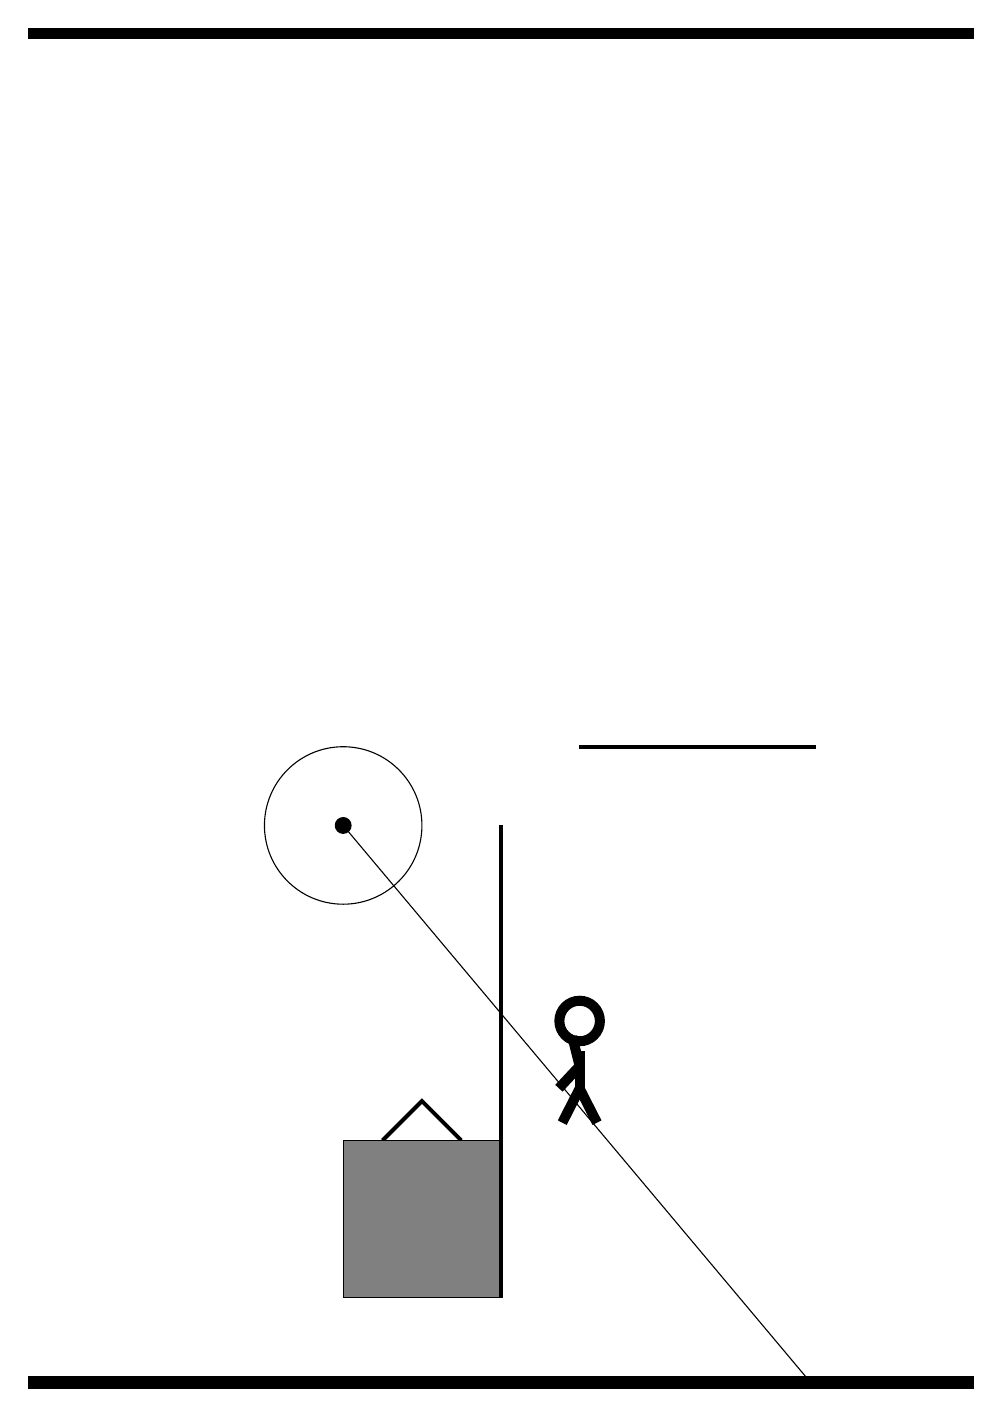
\begin{tikzpicture}
				\draw[fill=black] (-2, 14) rectangle (10, 14.125);
				
				\draw (2,4) circle (1);
				\draw[fill=black] (2,4) circle (0.1);
				\draw (8,-3.15) -- (2,4);
				
				\draw[line width=0.5mm](2.5,0) --  (3,0.5) -- (3.5,0);
				\draw[fill=black!50] (2, 0) rectangle (4, -2);
				
				\draw[line width = 0.5mm] (5,5) -- (8,5);
				\centerarc[line width = 0.5mm](5,4)(90:180:1);
				\draw[line width = 0.5mm] (4,4) -- (4,-2);
				\centerarc[line width = 0.5mm](5,-2)(180:360:1);
				
				\node at (5, 1) {\scriptsize \Strichmaxerl[10][47][104]};
				
				\draw[fill=black] (-2, -3) rectangle (10, -3.15);
			\end{tikzpicture}
		\end{subfigure}
		\hfill
		\begin{subfigure}[b]{0.48\textwidth}
			\caption{Figure 2}
			\centering
			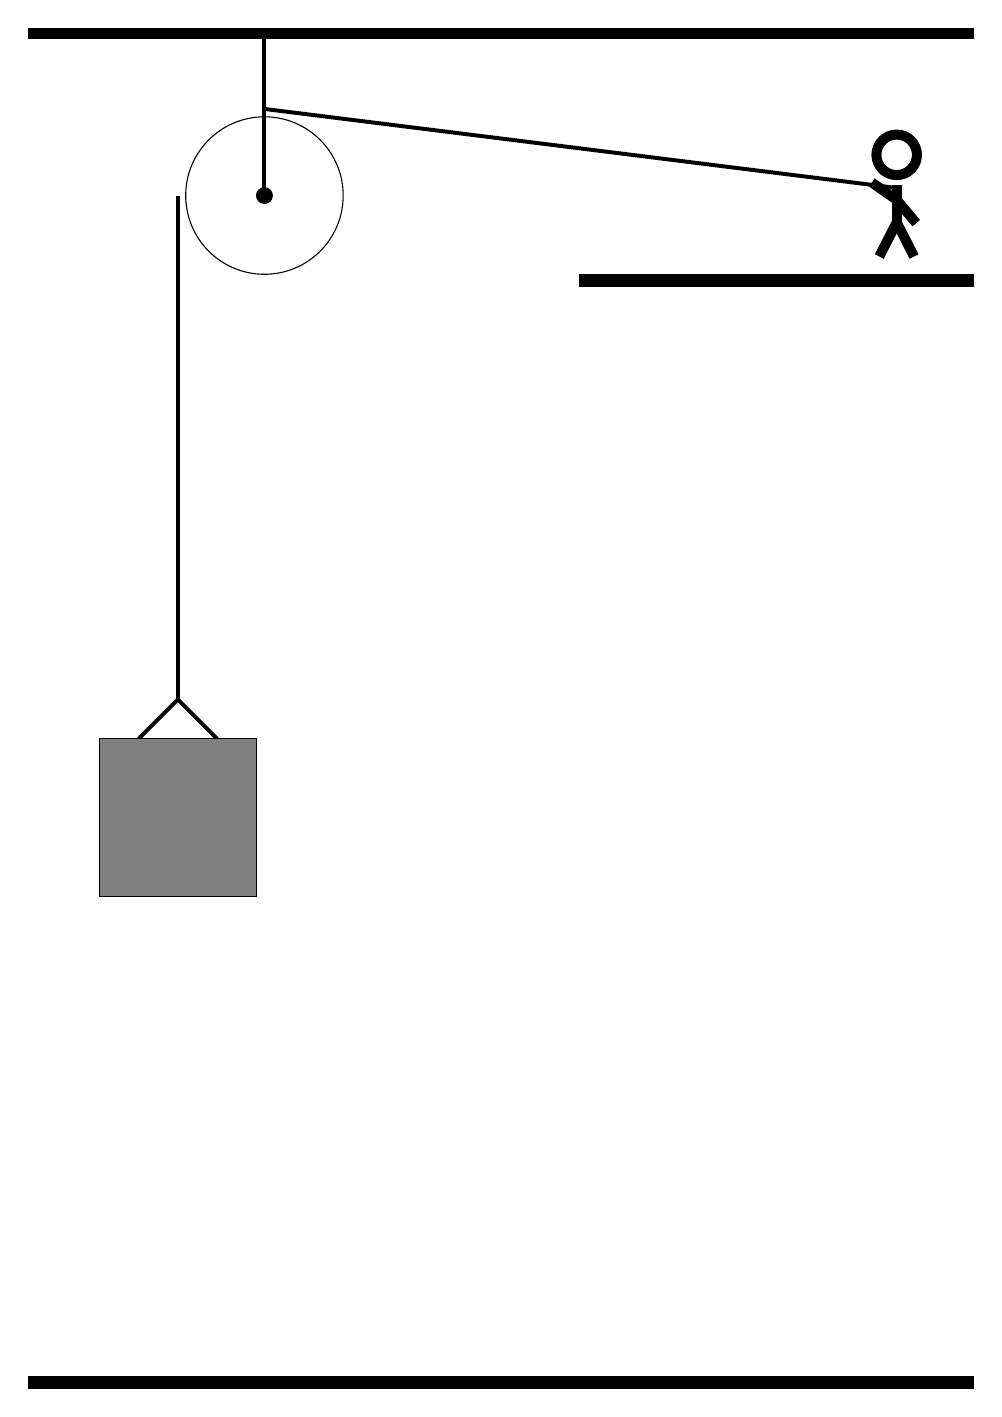
\begin{tikzpicture}
				\draw[fill=black] (-2, 14) rectangle (10, 14.125);
				
				\draw (1, 12) circle (1);
				\draw[fill=black] (1, 12) circle (0.1);
				\draw[line width=0.5mm] (1, 14) -- (1, 12);
				
				\draw[line width=0.5mm](-0.6, 5.1) --  (-0.1, 5.6) -- (0.4, 5.1);
				\draw[fill=black!50] (-1.1, 5.1) rectangle (0.9, 3.1);
				
				\draw[line width=0.5mm](-0.1, 12) -- (-0.1, 5.6);
				\centerarc[line width=0.5mm](1, 12)(90:180:1.1)
				\draw[line width=0.5mm](1, 13.1) -- (9, 12.1);
				
				\node at (9, 12) {\scriptsize \Strichmaxerl[10][-35][-50]};
				\draw[fill=black] (5, 11) rectangle (10, 10.85);
				
				\draw[fill=black] (-2, -3) rectangle (10, -3.15);
			\end{tikzpicture}
		\end{subfigure}
	\end{figure}
		\vspace*{\fill}
\end{document}